\section{Mininet BGP LAB}
\subsection{}
The address is \texttt{192.168.1.1}.

\subsection{}
The routing table consists of a list of pathways for the way to each
each network as shown:
\begin{center}
    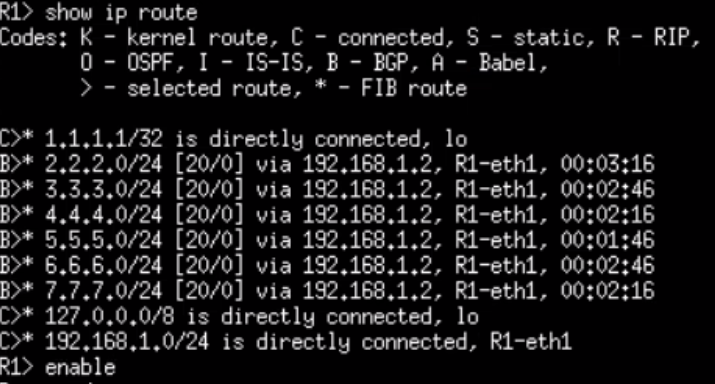
\includegraphics[width=1.2 \textwidth]{resources/q4-1.png}\centering
\end{center}
It appears all of the routes are through \texttt{192.168.1.2},
accept the loopback connection, and the \texttt{192.168.1.0} device.\\
Different entries in the table are controled by different applications or methods:
\texttt{1.1.1.1}, loopback and \texttt{192.168.1.0} have been
added to the table since they are directly connected to the device,
while the rest of the entries in the table have been added by the BGP protocol.\\
The timestamp at the end of the BGP entries shown when BGP has added the specific entry to the table.


\subsection{}
Different parts of the table are filled in different ways;
the entries for directly connected devices are added automatically - likely
by the operating system or an associated daemon,
while the indirect routings marked with 'B' have been added by the local
BGP application (\texttt{bgpd}).\\
Generally - different enties in the table are inserted from different sources,
and each such source might add it's own entries based on how the specific protocol is defined.



\subsection{}
The data stored in the BGP table represents the next hop, which is the next
router on our network where we want our messages to be sent.
In our case, where AS1 is only connected to AS2, all our messages need to be
routed through AS2 to reach their destinations.
We can also see the path the packets need to go through in the net\dots

\subsection{}
The route from \texttt{R1} to \texttt{R5} shown
in the BGP table is shown as "\texttt{0 2 3 4 5 i}",
which means the route goes through \texttt{R3} and \texttt{R4}.\\
The reason the path going through \texttt{R6} and \texttt{R7} is not
shown is because it is was not considered an optimal path by BGP
\footnote{The metric is determined by the
configuration - the number of hops between AS's and the weight/cost of each hop}
and hence it was not saved.\\

\subsection{}
\texttt{R2} shows two routes to \texttt{R5},
one through \texttt{R6} and the other through \texttt{R3};
the one through \texttt{R3} is the one used, as it is the shortest one
considering the AS-hop-counte metric.

\subsection{}
If all metrics are equal to zero, then the routing is dicated by taking the
shortest path in terms of the number of hops between AS's, if  that does not break
the tie - then random / lexicographic selection is used.

\subsection{}
It seems the path in the bgp table from texttt{R5} to texttt{R1} \texttt{0 4 7 6 2 1 3 1 i}.
\begin{center}
    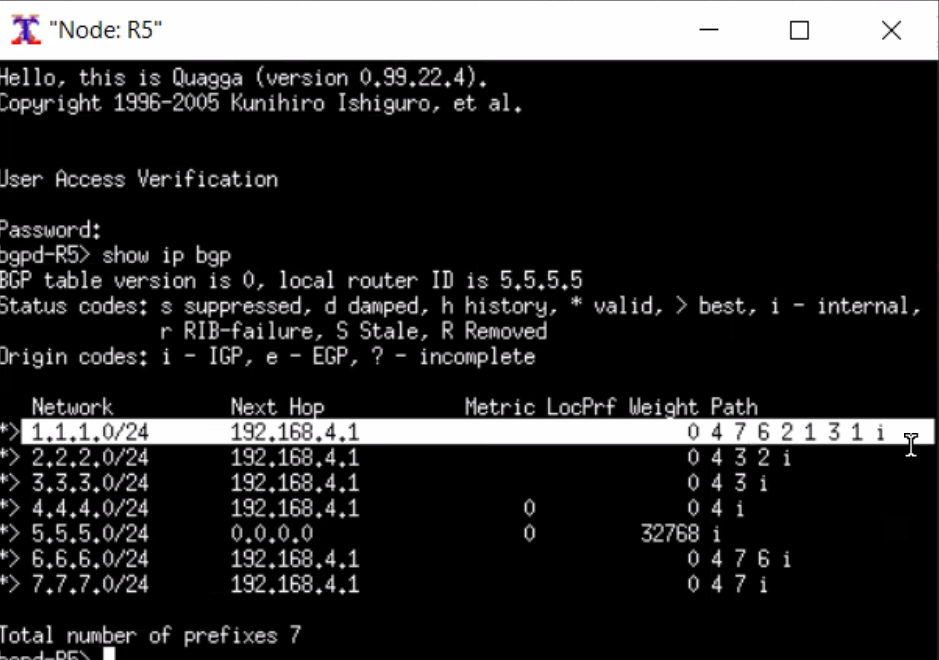
\includegraphics[width=1.2 \textwidth]{resources/q4-2.png}\centering
\end{center}

\subsection{}
The AS manager added the prefix \texttt{3 1} to 
\begin{center}
    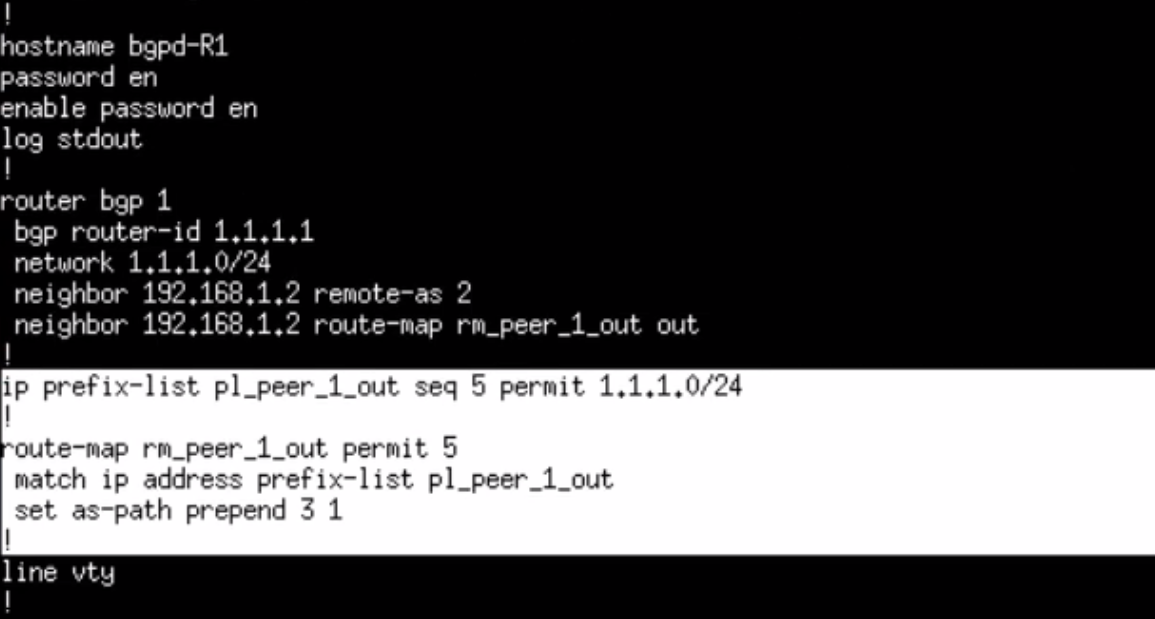
\includegraphics[width=1.2 \textwidth]{resources/q4-3.png}\centering
\end{center}

\subsection{}
\begin{center}
    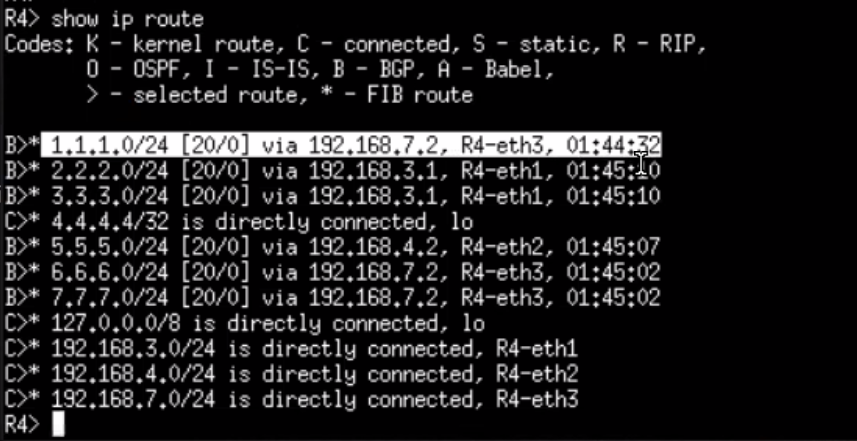
\includegraphics[width=1.2 \textwidth]{resources/q4-4.png}\centering
\end{center}
 we can see in the line 192.168.7.0 is directly connected, R4-
